\documentclass[12pt,titlepage]{article}
\usepackage[ngerman]{babel}
\usepackage{color}
\usepackage[a4paper,lmargin={3cm},rmargin={3cm},
tmargin={2.5cm},bmargin = {2.5cm}]{geometry}
\usepackage{graphicx}
\usepackage{amssymb}
\usepackage{amsthm}
\usepackage{graphicx}
\usepackage{cite}
\def\theequation{\thesection.\arabic{equation}}
\linespread{1.5}
\usepackage{amsmath}
\usepackage{mathtools}
\numberwithin{equation}{section}
\usepackage[utf8]{inputenc}
\usepackage[T1]{fontenc}
\usepackage{subcaption}
\usepackage{chngcntr}
\counterwithin{figure}{section}
\usepackage{float}
\usepackage{pdfpages}
\usepackage{hyperref}
\begin{document}



%Title Seite
\begin{titlepage}
    \title{Student Competition- Aufgabe 2}
    \date{30.06.2023}
    \author{Constantin Lüth - Dante Bartoli\\ Gruppenname: Kruskal }
    \maketitle
\end{titlepage}
 
\pagenumbering{Roman}
\setcounter{page}{2} 
\tableofcontents
\newpage


\pagenumbering{arabic}
%Hier Einleitung reinschreiben
\section{Aufgabe}
Ein Erdbeerbauer besitzt zwei Felder, auf denen er jeweils Erdbeeren anpflanzt. Wegen einer
Durre sind schon sehr viele Pflanzen gestorben, weshalb er die restlichen Pflanzen nun bewässern
möchte. Die Bewässerung soll so erfolgen, dass möglichst wenig Wasserschlauch verlegt werden
muss. Die Schläuche können sich beliebig verzweigen und eine Wasserabgabe kann an jedem
beliebigen Punkt des Schlauches erfolgen.

\section{Aufgabenteil a}
Das kleine Feld (Feld 1) misst 10 x 10. Leider haben hier nur 15 Pflanzen uberlebt. Ihre ¨
Positionen sind in Abbildung 1 dargestellt. Die Koordinaten finden Sie in der Excel-Datei
”Erdbeerfelder.xlsx” im Datenblatt ”Feld 1”.

\subsection{Aufgabenteil a1}
Aufgabe: Wie verlaufen die Schläuche, wenn sich die Wasserpumpe genau bei Pflanze 1 befindet?
\subsubsection*{Idee 1}

Wir verwenden einen >>minimal spannenden Baum<<, um alle Pflanzen mit minimalen Wasserschlauchmetern zu bewässern.

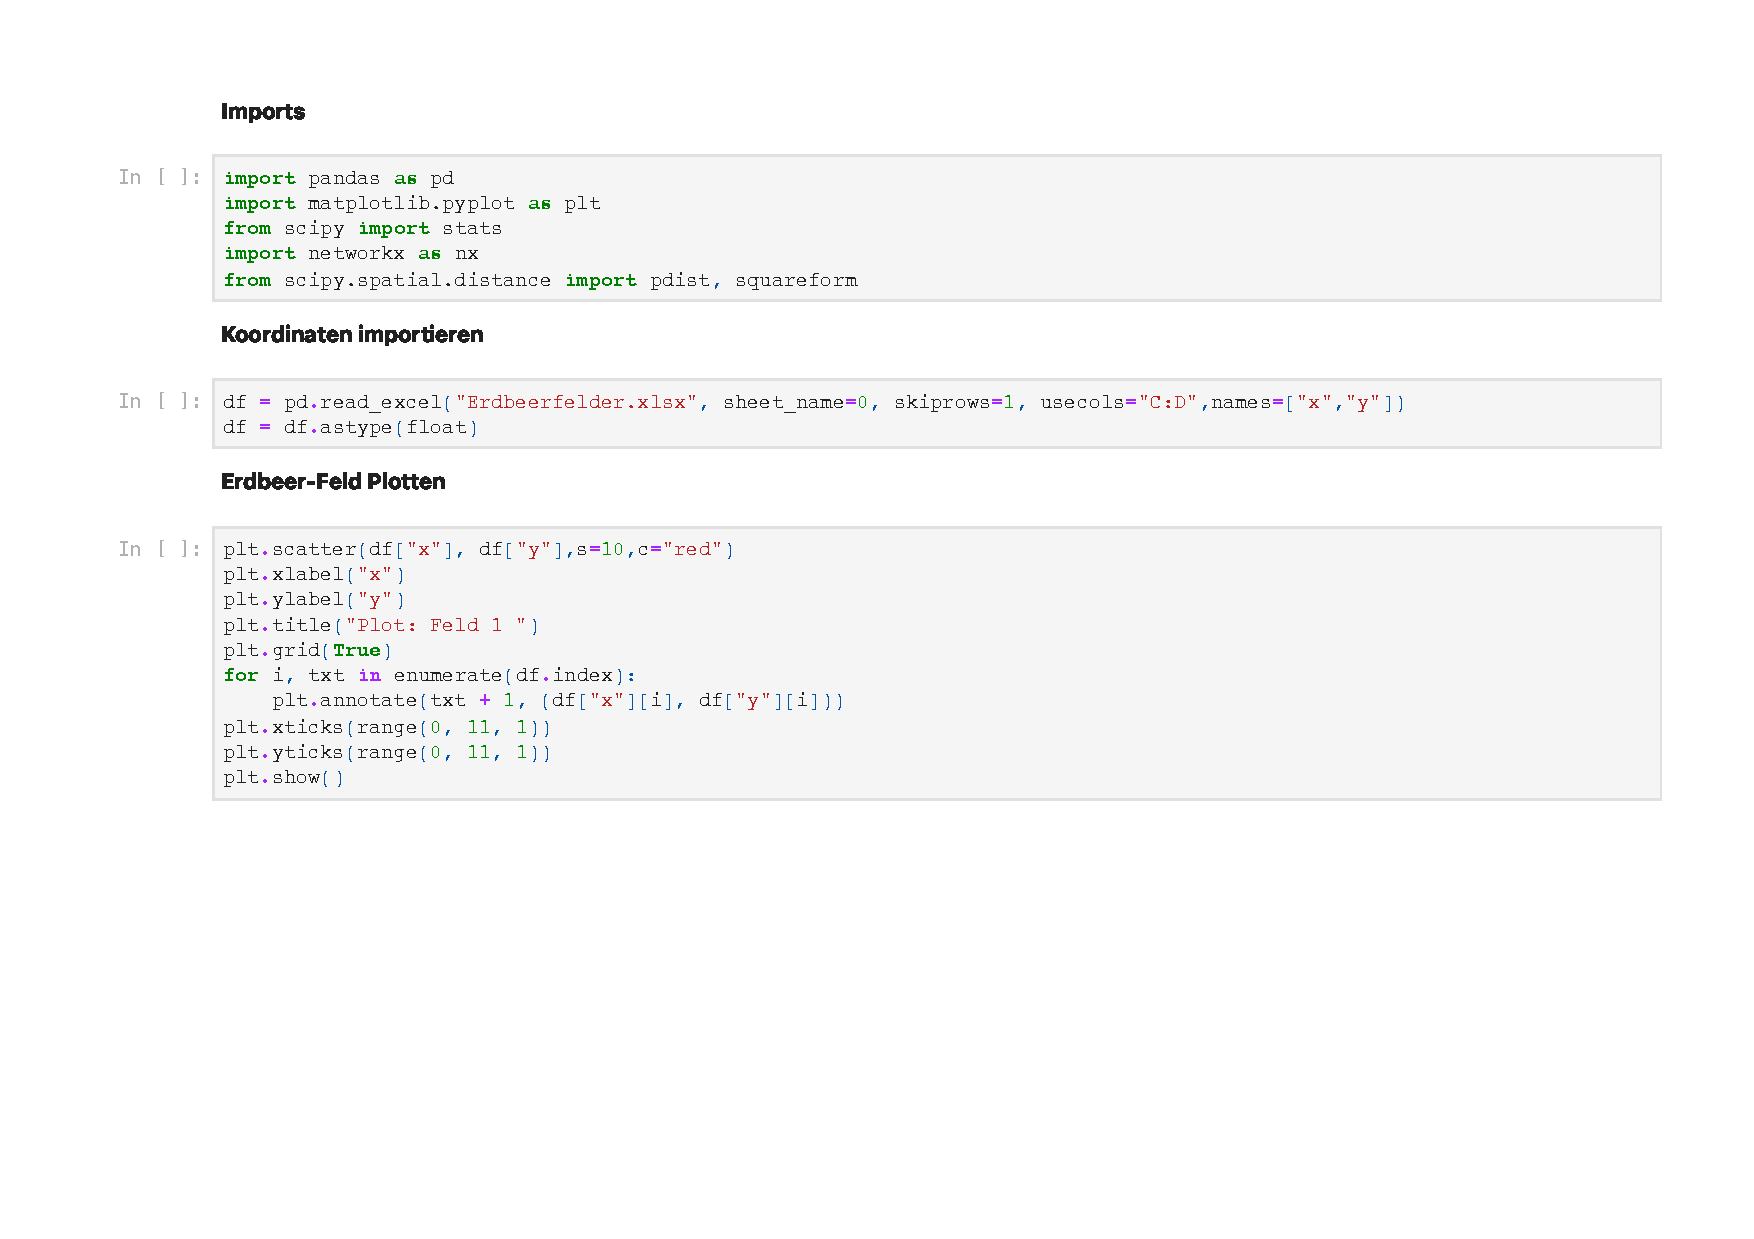
\includepdf[pages={1,2},nup=1x2]{/Users/constantin/git/Machine-Learning/a1.pdf}
\includepdf[pages={3,4},nup=1x2]{/Users/constantin/git/Machine-Learning/a1.pdf}

\subsubsection*{Ergebnis 1}

Wir erhalten einen minimal spannenden Baum mit einer Länge von 31.41 Meter.

\subsection{Aufgabenteil a2}
Aufgabe: Was ändert sich an Ihrer Lösung, wenn sich die Wasserpumpe genau bei Pflanze 2 befindet?
\\ \\
 \noindent Nichts, da es für den minimal-spannenden-Baum unerheblich ist, wo sich die Wasserpumpe befindet (vgl. Abbildung \ref{fig:a2}). 
Die Schläuche bleiben in der gleichen Position wie in Aufgabe a1.

\begin{figure}[H]
	\centering
	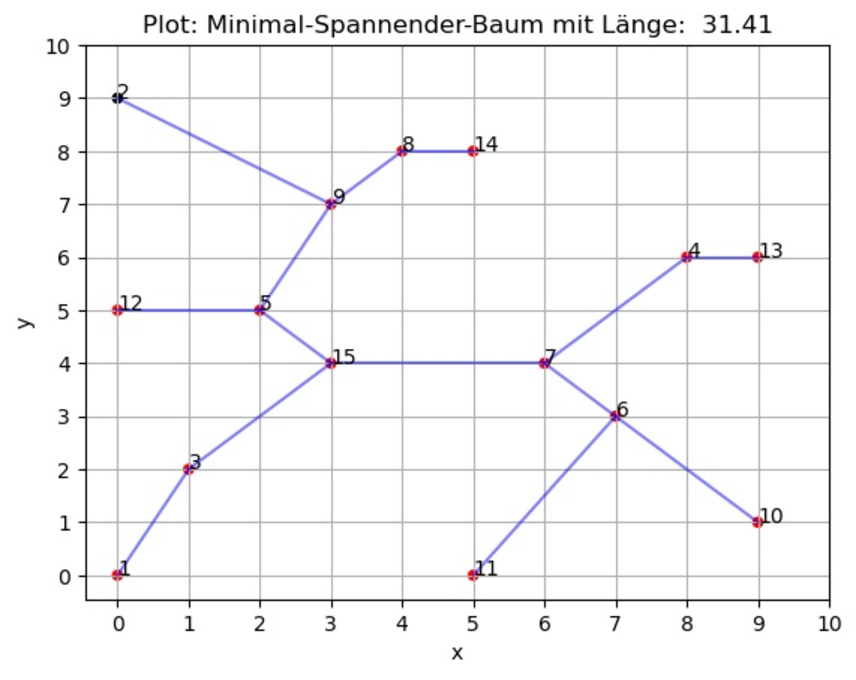
\includegraphics[width=0.95\textwidth]{/Users/constantin/git/Machine-Learning/Bilder/a2.pdf}
	\caption{Minimal spannender Baum (Pumpe im Punkt 2) }
	\label{fig:a2}
\end{figure}

\subsection{Aufgabenteil a3}
Aufgabe: Finden Sie eine möglichst gute Lösung fur den Fall, dass sich genau bei Pflanze 1 und in Koordinatenposition (10/10) eine Wasserpumpe befindet.

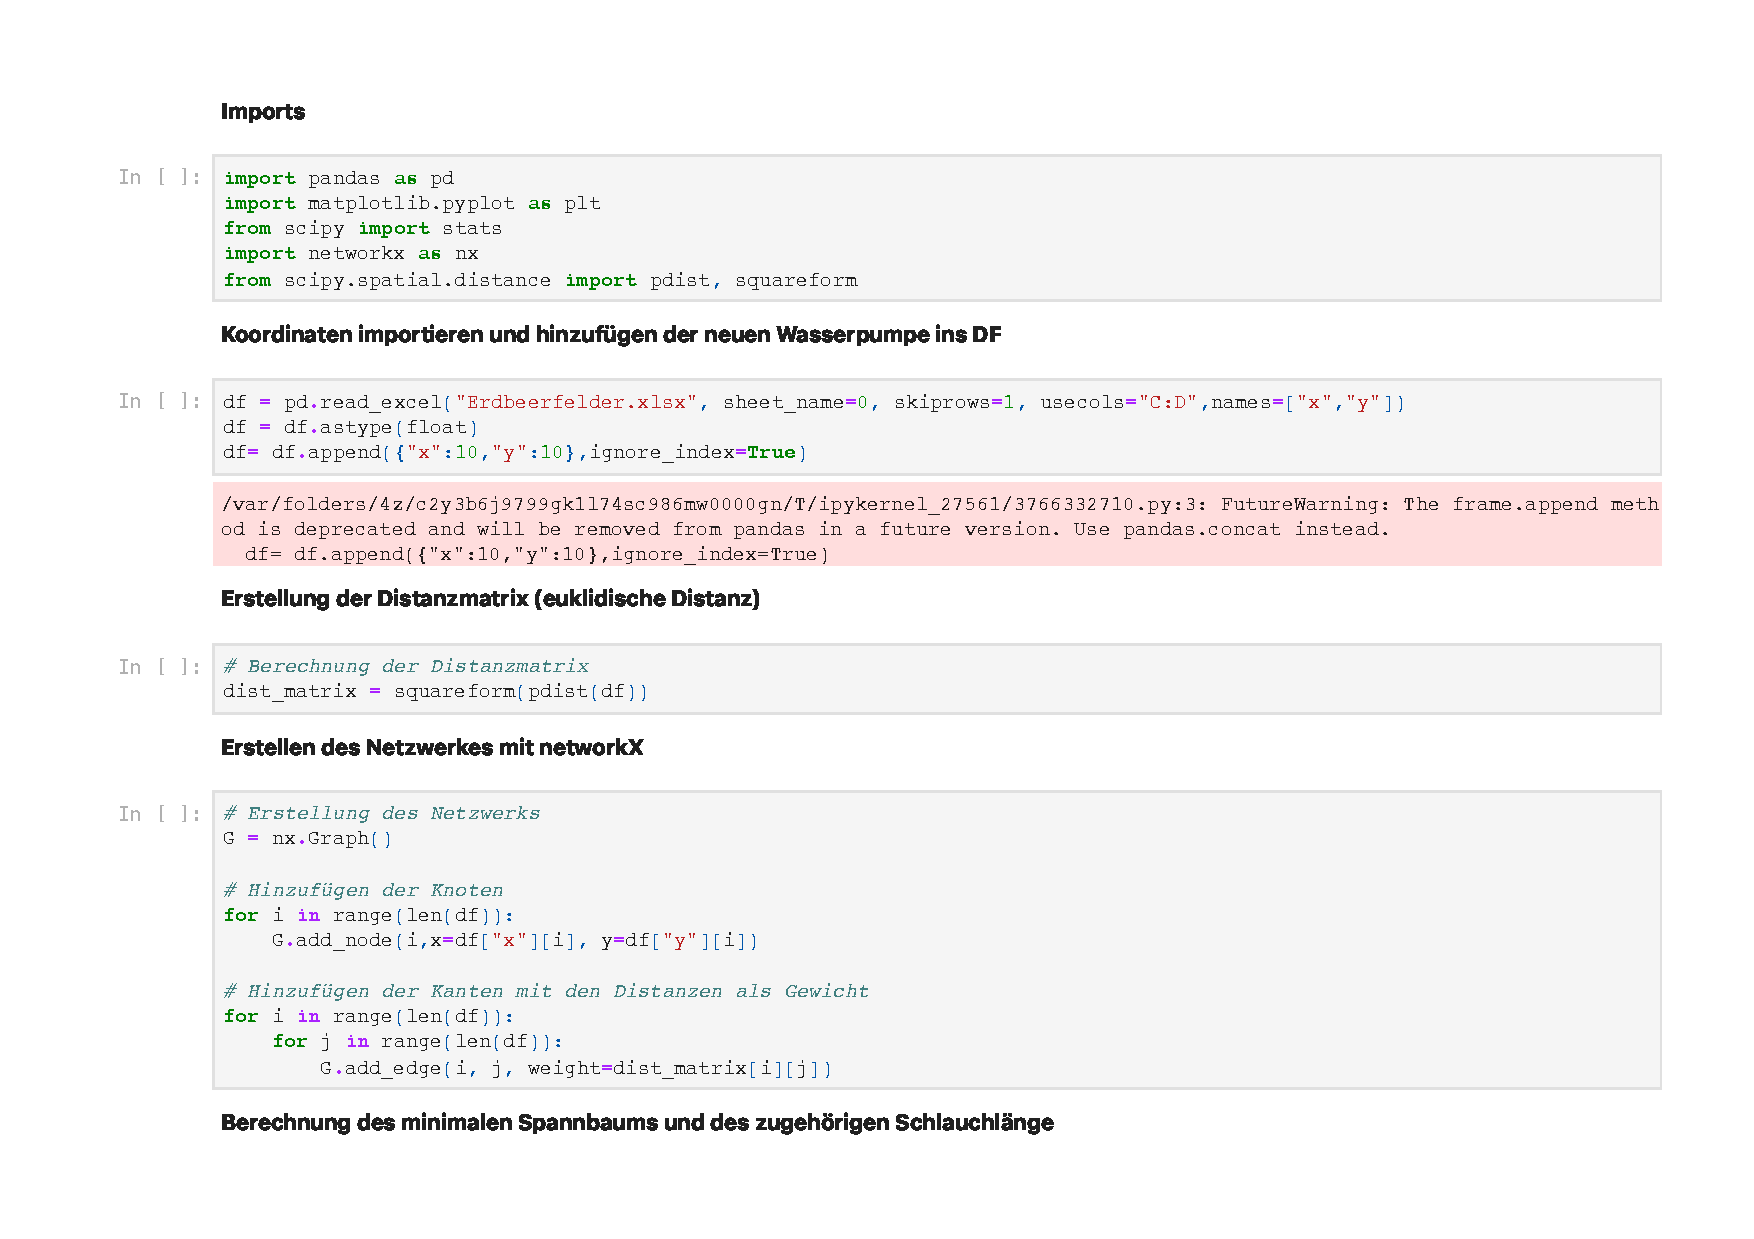
\includepdf[pages={1-2},nup=1x2]{/Users/constantin/git/Machine-Learning/a3.pdf}
\includepdf[pages={3-4},nup=1x2]{/Users/constantin/git/Machine-Learning/a3.pdf}
\includepdf[pages={5-6},nup=1x2]{/Users/constantin/git/Machine-Learning/a3.pdf}
\includepdf[pages={7-8},nup=1x2]{/Users/constantin/git/Machine-Learning/a3.pdf}
\includepdf[pages={9-10},nup=1x2]{/Users/constantin/git/Machine-Learning/a3.pdf}
\includepdf[pages={11-12},nup=1x2]{/Users/constantin/git/Machine-Learning/a3.pdf}
\includepdf[pages={13-14},nup=1x2]{/Users/constantin/git/Machine-Learning/a3.pdf}
\includepdf[pages={15},nup=1x2]{/Users/constantin/git/Machine-Learning/a3.pdf}


\subsection{Aufgabenteil a4}
Aufgabe: Finden Sie eine möglichst gute Lösung, wenn zwei Wasserpumpen benutzt werden sollen
und sich diese an beliebiger Stelle befinden können. Beschreiben und begrunden Sie Ihr
Vorgehen bei der Standortwahl fur die Wasserpumpen und bei der Entscheidungsfindung
fur die Verlegung der Schläuche genau.

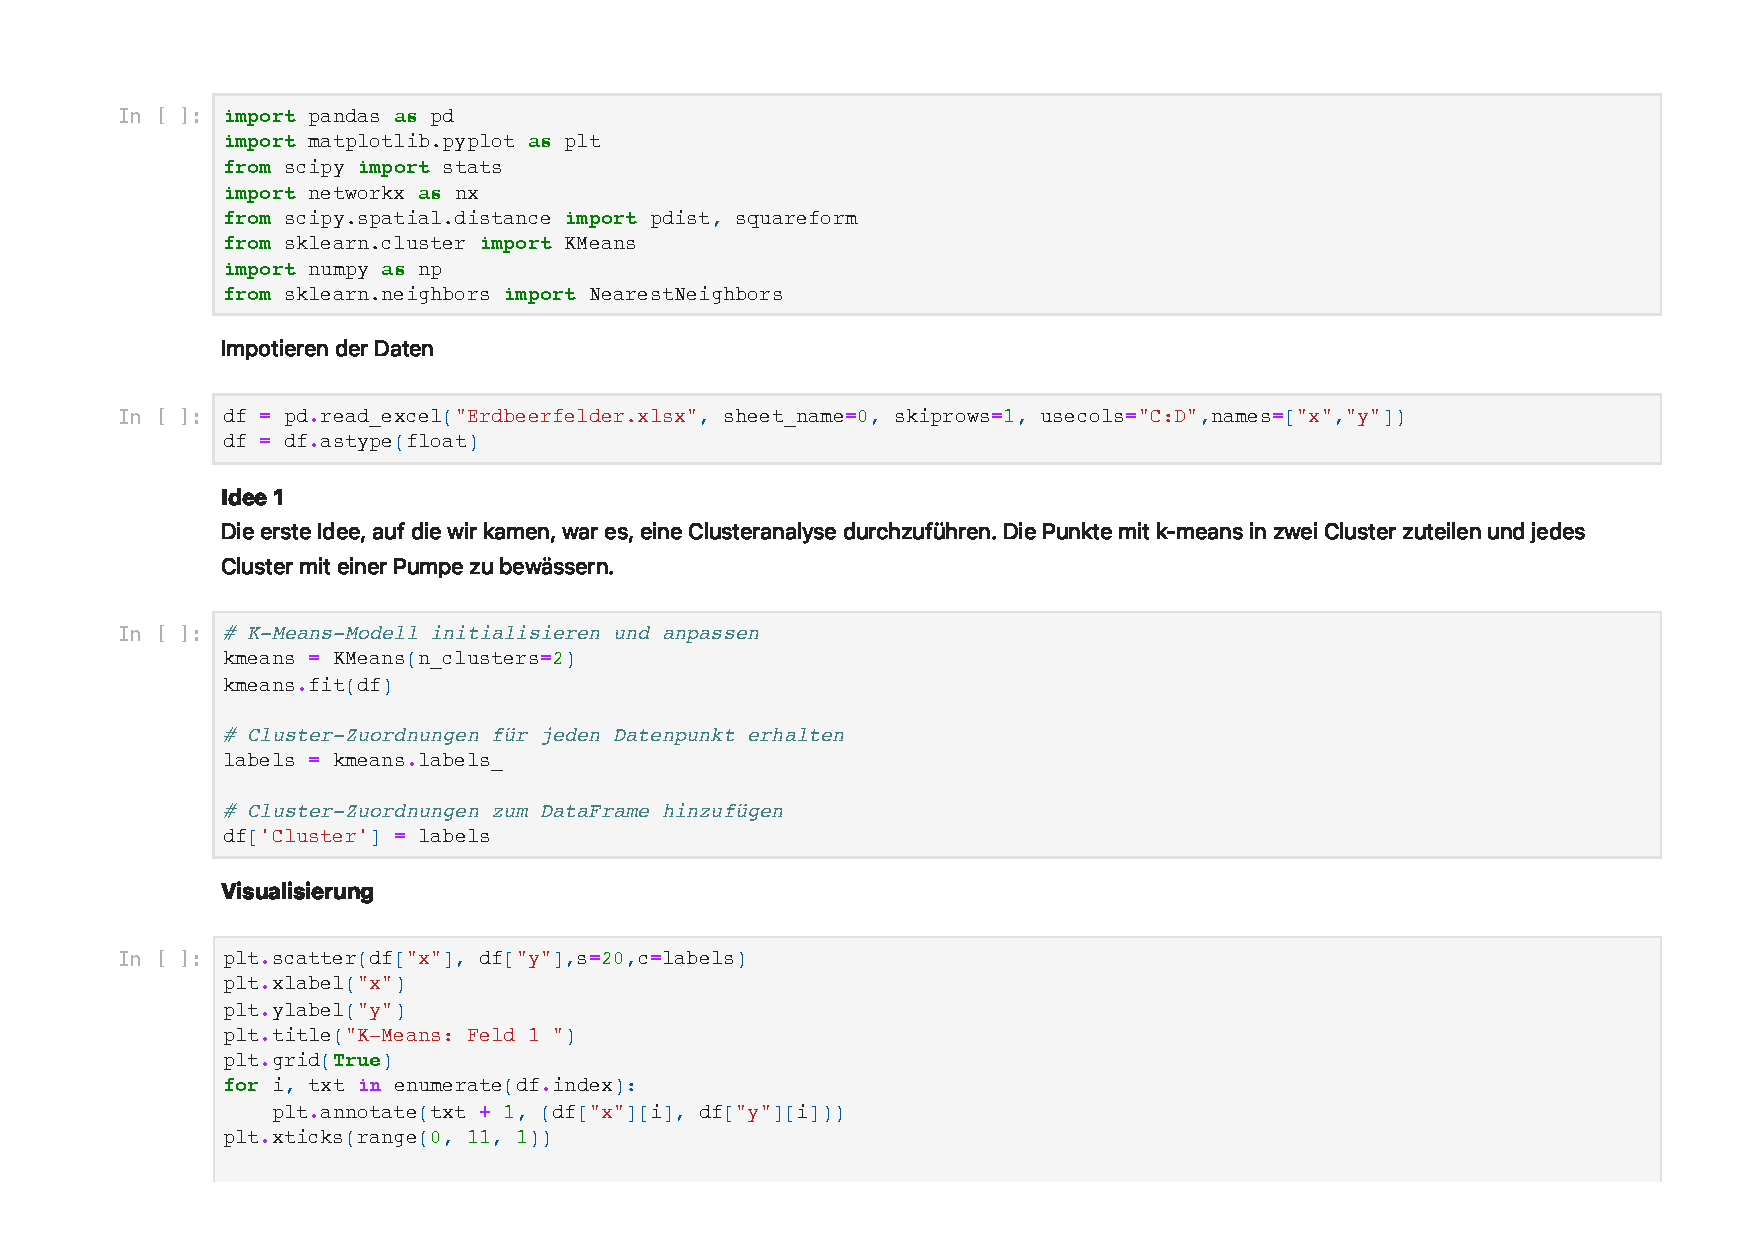
\includepdf[pages={1-2},nup=1x2]{/Users/constantin/git/Machine-Learning/a4.pdf}
\includepdf[pages={3-4},nup=1x2]{/Users/constantin/git/Machine-Learning/a4.pdf}
\includepdf[pages={5-6},nup=1x2]{/Users/constantin/git/Machine-Learning/a4.pdf}
\includepdf[pages={7-8},nup=1x2]{/Users/constantin/git/Machine-Learning/a4.pdf}
\includepdf[pages={9},nup=1x2]{/Users/constantin/git/Machine-Learning/a4.pdf}


\section{Aufgabenteil b}
Das große Feld (Feld 2) misst 100 x 100. Hier haben 150 Pflanzen uberlebt. Ihre Positionen ¨
sind in Abbildung 2 gegeben, die Koordinaten finden Sie im Datenblatt ”Feld 2” der ExcelDatei ”Erdbeerfelder.xlsx”. Finden Sie auch hier eine möglichst gute Lösung, wenn zwei
Wasserpumpen benutzt werden sollen und sich diese an beliebiger Stelle befinden können.
Beschreiben und begrunden Sie Ihr Vorgehen bei der Standortwahl für die Wasserpumpen ¨
und bei der Entscheidungsfindung fur die Verlegung der Schläuche. Wie haben Sie Ihr Vorgehen im Vergleich zu a4) angepasst?

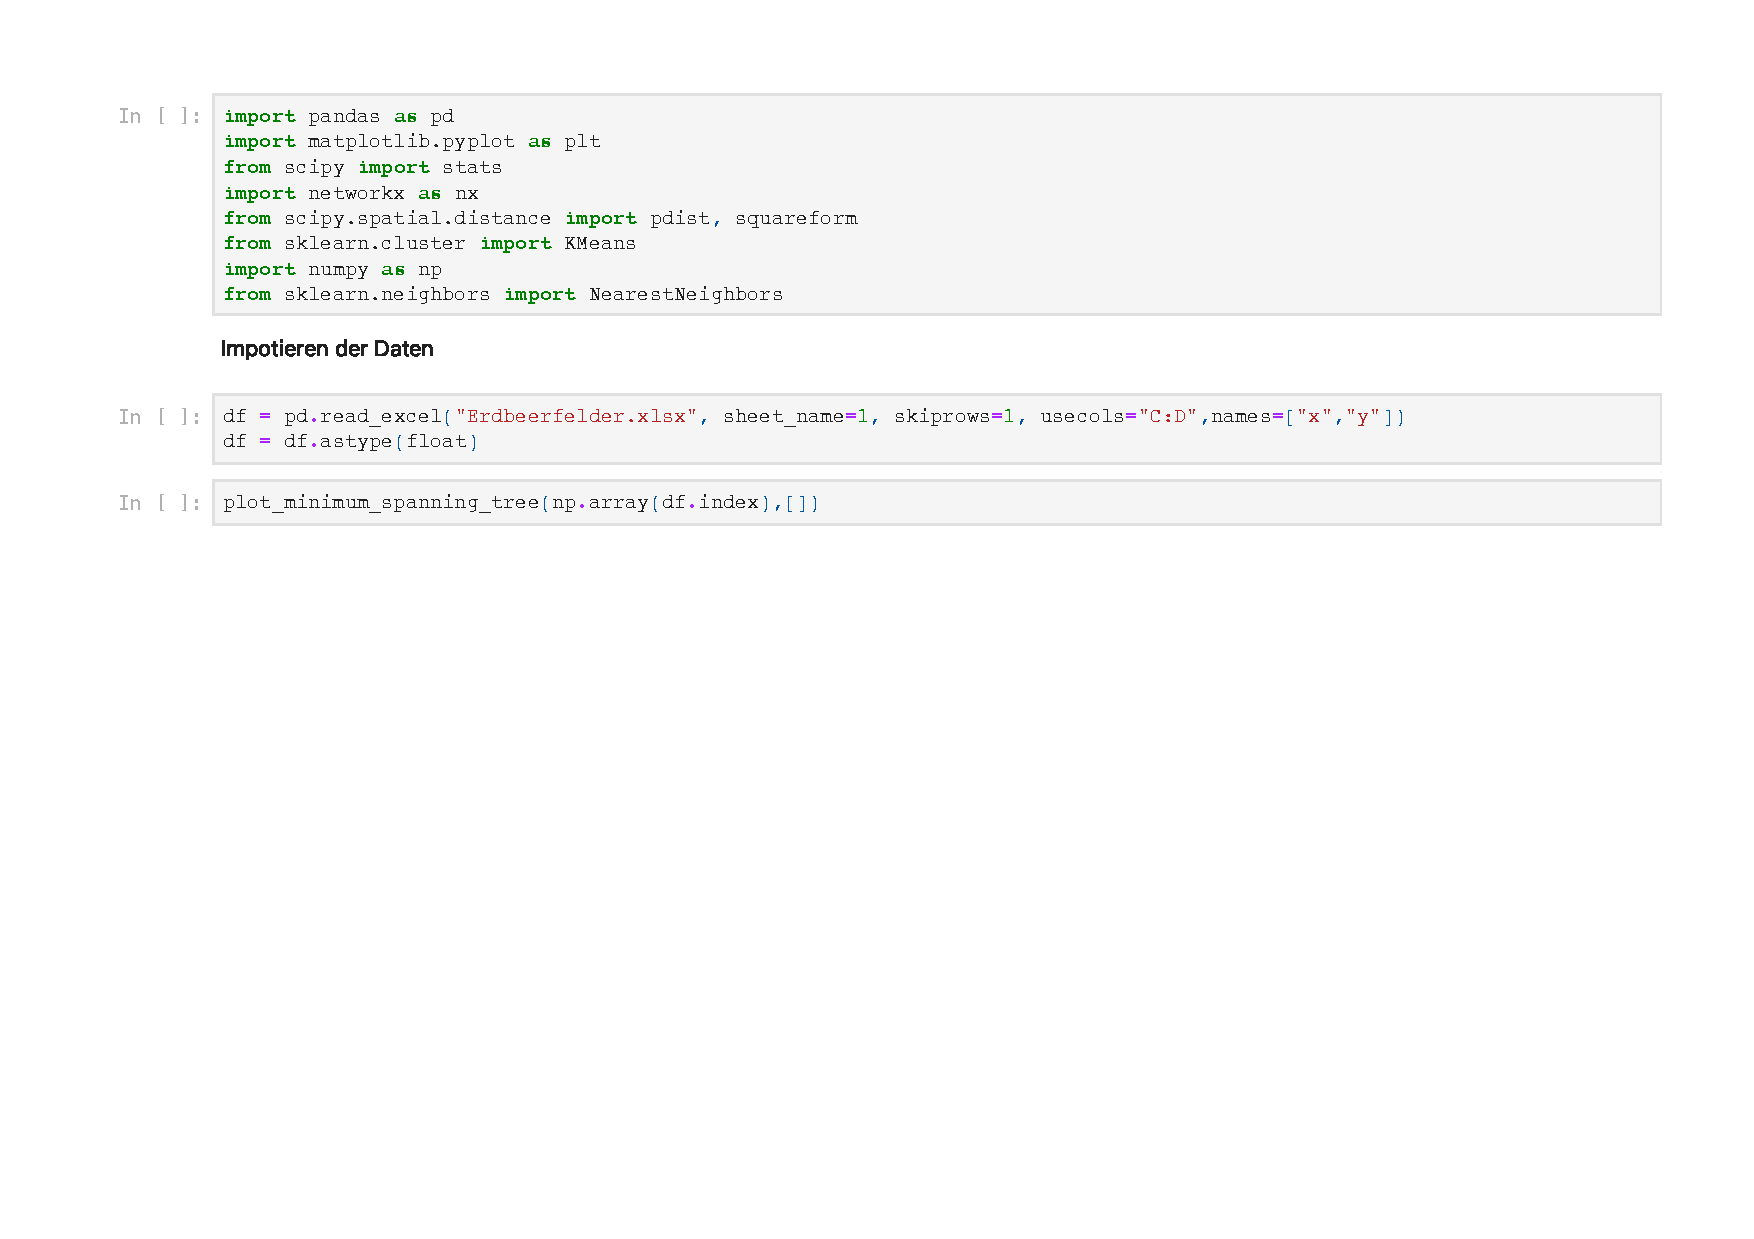
\includepdf[pages={1-2},nup=1x2]{/Users/constantin/git/Machine-Learning/b.pdf}
\includepdf[pages={3-4},nup=1x2]{/Users/constantin/git/Machine-Learning/b.pdf}
\includepdf[pages={5-6},nup=1x2]{/Users/constantin/git/Machine-Learning/b.pdf}

\section{Bibliotheken}
\begin{table}[h]
    \centering
    \begin{tabular}{|l|l|}
    \hline
    \textbf{Bibliothek} & \textbf{URL} \\
    \hline
    Pandas & \url{https://pandas.pydata.org/} \\
    \hline
    Matplotlib & \url{https://matplotlib.org/} \\
    \hline
    SciPy & \url{https://scipy.org/} \\
    \hline
    scikit-learn & \url{https://scikit-learn.org/stable/} \\
    \hline
    NumPy & \url{https://numpy.org/} \\
    \hline
    NetworkX & \url{https://networkx.org/} \\
    \hline
    \end{tabular}
    \end{table}
    
\end{document}
